\def\figpath{tex/2_LC-Oszillator/pictures}
\graphicspath{{tex/2_LC-Oszillator/pictures/}}

\chapter{LC-Oszillator}
Das 2. Kapitel behandelt die Analyse der in Abb. \ref{fig_Kap2_01:Oszillator} gezeigten Oszillatorschaltung.

\begin{figure}[H]
    \centering
    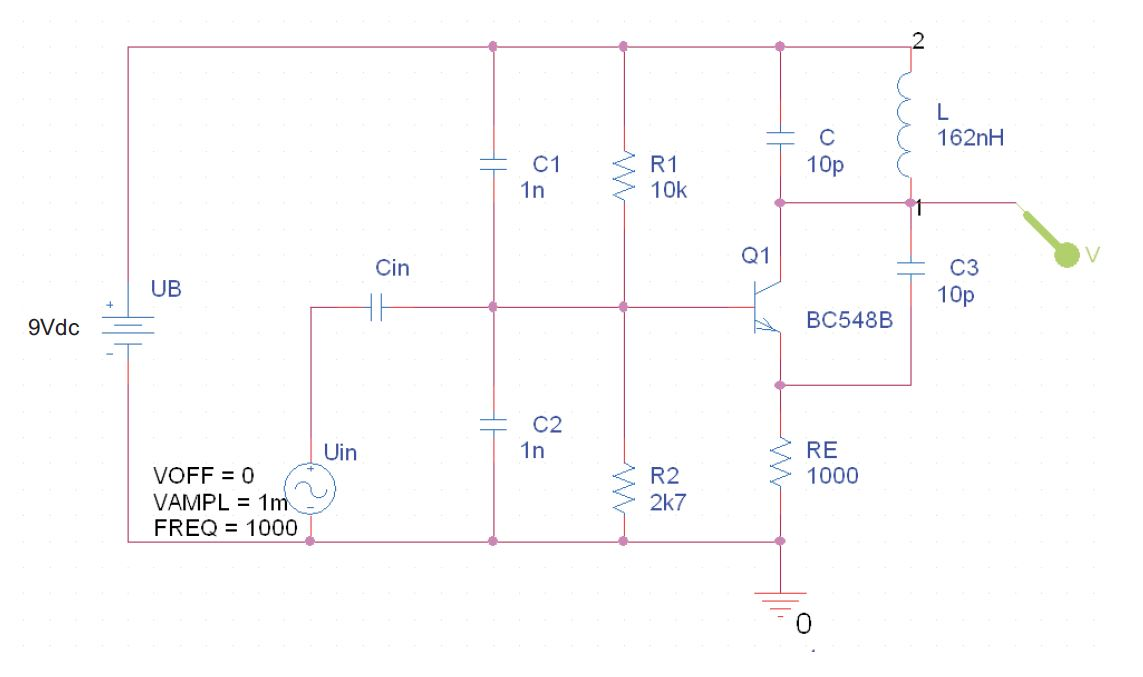
\includegraphics[width = \textwidth]{\figpath/Oszillatorschaltung.jpg}
    \caption{Oszillatorschaltung}
    \label{fig_Kap2_01:Oszillator}
\end{figure}

\section{Schwingbedingung}
Zuerst soll auf Basis des Kleinsignalersatzschaltbildes die Resonanzfrequenz berechnet werden. Hierbei dürfen lt. Praktikumsskript die Kapazitäten $C_1$ und $C_2$ als unendlich angenommen werden. Außerdem sind die parasitären Kapazitäten des Transistors lt. Abb. \ref{fig_Kap2_02:parasit} zu berücksichtigen.

\begin{figure}[H]
    \centering
    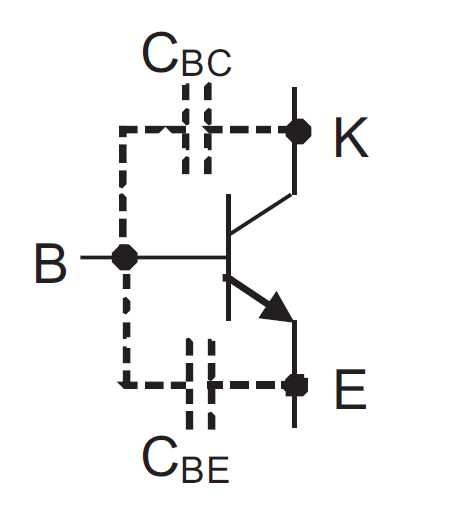
\includegraphics[width = 0.3\textwidth]{\figpath/parasit.jpg}
    \caption{Oszillatorschaltung}
    \label{fig_Kap2_02:parasit}
\end{figure}

Das KSESB der Oszillatorschaltung sieht folgendermaßen aus:

\begin{figure}[H]
	\centering
	\def\svgwidth{0.8\textwidth}
	\input{\figpath/KSESB.pdf_tex}
	\caption{KSESB der Oszillatorschaltung} 
	\label{fig:01_QStatAufbau} 
\end{figure}

Fasst man die relevanten Bauteile zu zwei Ersatzimpendazen

\begin{equation}
    \underline{Z}_1 = \frac{1}{\underline{Y}_1} = \frac{1}{\frac{S}{B}+\frac{1}{R_E}+j  \omega C_{BE}}
\end{equation}

\begin{equation}
    \underline{Z}_2 = \frac{1}{\underline{Y}_2} = \frac{1}{\frac{1}{j\omega L}+j \omega \left( C_{BC} + C \right)}
\end{equation}

zusammen, so lässt sich die Schaltung vereinfacht darstellen:

\begin{figure}[H]
	\centering
	\def\svgwidth{0.6\textwidth}
	\input{\figpath/KSESB2.pdf_tex}
	\caption{Vereinfachtes KSESB der Oszillatorschaltung} 
	\label{fig:01_QStatAufbau} 
\end{figure}

Laut der Kirchhoffschen Maschenregel kann nun folgender Ausdruck gebildet werden:

\begin{equation}
    u_{BE} \cdot \left( 1 + \frac{S + \underline{Y}_1}{j \omega C_3} + \frac{\underline{Y}_1}{\underline{Y}_2} \right) = 0
\end{equation}

Setzt man nun die Ausdrücke der Ersatzadmittanzen ein folgt:
\begin{equation}
    u_{BE} \cdot \left( 1 + \frac{S + \frac{S}{B}+\frac{1}{R_E}+j  \omega C_{BE}}{j \omega C_3} + \frac{\frac{S}{B}+\frac{1}{R_E}+j  \omega C_{BE}}{\frac{1}{j\omega L}+j \omega \left( C_{BC} + C \right)} \right) = 0
\end{equation}

Die Steuergröße des Oszillators, die Basis-Emitterspannung $u_{BE}$, darf naturgemäß nicht verschwinden, womit sich die Schwingbedingung im komplexen Zahlenraum ergibt:

\begin{equation}
    1 + \frac{S + \frac{S}{B}+\frac{1}{R_E}+j  \omega C_{BE}}{j \omega C_3} + \frac{\frac{S}{B}+\frac{1}{R_E}+j  \omega C_{BE}}{\frac{1}{j\omega L}+j \omega \left( C_{BC} + C \right)} = 0
\end{equation}

Betrachtet man nun den Real- und Imaginärteil obiger Gleichung einzeln, erhält man 2 reelle Schwingbedingungen, was mithilfe des Computeralgebraprogramms \textit{MAXIMA} hergeleitet wurde.\\
Für den Realteil gilt:

\begin{equation}
\label{glng_01}
    1 + \frac{C_{BE}\omega}{\omega (C_{BC} + C) - \frac{1}{\omega L}} + \frac{C_{BE}}{C_3} = 0
\end{equation}

Für den Imaginärteil ergibt sich folgende Gleichung:
\begin{equation}
    \label{glng_03}
    -\frac{\frac{S}{B}+\frac{1}{R_E}}{\omega(C_{BC} + C)-\frac{1}{\omega L}} - \frac{S\left(\frac{1}{B} + 1\right) + \frac{1}{R_E}}{\omega C_3} = 0
\end{equation}

Der variable Emitterwiderstand $R_E$ kommt in Gleichung \ref{glng_01} nicht vor, wodurch sich ein Ausdruck für die Resonanzkreisfrequenz aus einer quadratischen Gleichung finden lässt, wobei natürlich die negative Lösung verworfen wird: 

\begin{equation}
    \label{glng_02}
    \omega = \sqrt{\frac{C_{BE} + C_3}{\left( \left( C_{BC} + C_3 + C\right)C_{BE} + C_3 C_{BC} + CC_3 \right) L}}
\end{equation}

Setzt man nun die Lösung \ref{glng_02} in Gleichung \ref{glng_03} ein, lässt sich ein Ausdruck für den variablen Widerstand $R_E$ in Abhängigkeit der Steilheit $S$ des Transistors im jeweiligen Arbeitspunkt finden:

\begin{equation}
    R_E = \frac{B \cdot C_3}{S \cdot \left( B C_{BE} - C_3\right)}
\end{equation}

In Tab. \ref{tab_Kap2_01:Bauteilwerte} werden die aus dem in Abb. \ref{fig_Kap2_01:Oszillator} gezeigten Schematic verwendeten Bauteilwerte und Werte der Versorgungsspannung aufgelistet. Für die parasitären Kapazitäten $C_{BE}$ und $C_{BC}$ wurden für die Berechnung die approximierten Werte aus dem Skriptum verwendet.

\begin{table}[H]
\centering
\begin{tabular}{|c|c|} \hline
Benennung & Größe \\ \hline
$U_B$ & \SI{9}{\volt} \\ \hline
$C$ & \SI{9}{\volt} \\ \hline
$C_1$ & \SI{1}{\nano\farad} \\ \hline
$C_2$ & \SI{1}{\nano\farad} \\ \hline
$C_3$ & \SI{10}{\pico\farad} \\ \hline
$C_{BC}$ & \SI{5}{\pico\farad} \\ \hline
$C_{BE}$ & \SI{10}{\pico\farad} \\ \hline
$L$ & \SI{162}{\nano\henry} \\ \hline
$R_1$ & \SI{10}{\kilo\ohm} \\ \hline
$R_2$ & \SI{2.7}{\kilo\ohm} \\ \hline
$R_E$ & \SI{1}{\kilo\ohm} \\ \hline

\end{tabular}
\caption{Bauteilwerte für Berechnung und Simulation}
\label{tab_Kap2_01:Bauteilwerte} 
\end{table}

Diese Werte in Gleichung \ref{glng_02} eingesetzt, ergeben die Resonanzkreisfrequenz bzw. Frequenz von:

\begin{equation}
    \omega = \SI{555.5}{\mega \radian \per \second}
\end{equation}

\begin{equation}
    f = \frac{\omega}{2 \cdot \pi} = \frac{\SI{555.5}{\mega \radian \per \second}}{2 \cdot \pi} = \SI{88.42}{\mega \hertz}
\end{equation}


\section{Simulation}
Das Schematic laut Abbildung \ref{fig_Kap2_05:LTSpiceSchematic} wurde in LTSpice nachgebildet.

\begin{figure}[H]
    \centering
    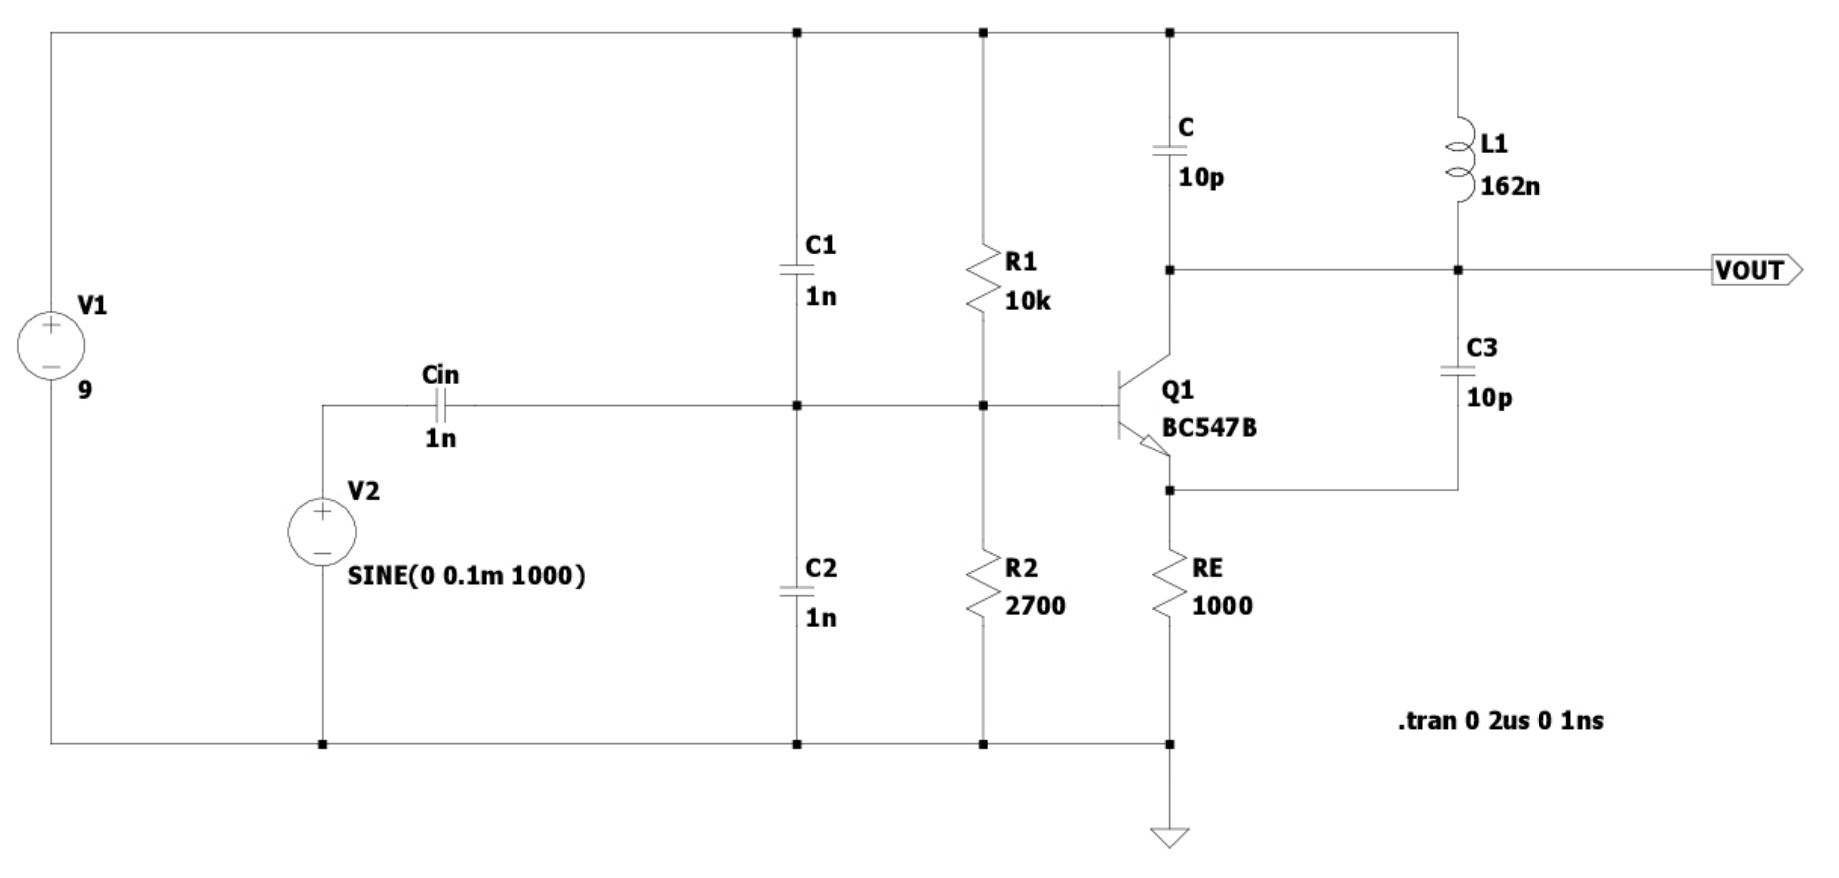
\includegraphics[width = \textwidth]{\figpath/LC_Oszillator_LTSpice.jpg}
    \caption{Oszillatorschaltung}
    \label{fig_Kap2_05:LTSpiceSchematic}
\end{figure}

Abbildung \ref{fig_Kap2_06:Einschw} zeigt den Einschwingvorgang der Oszillatorschaltung von 0 bis $\SI{2}{\micro\second}$. 

\begin{figure}[H]
	\centering \small
	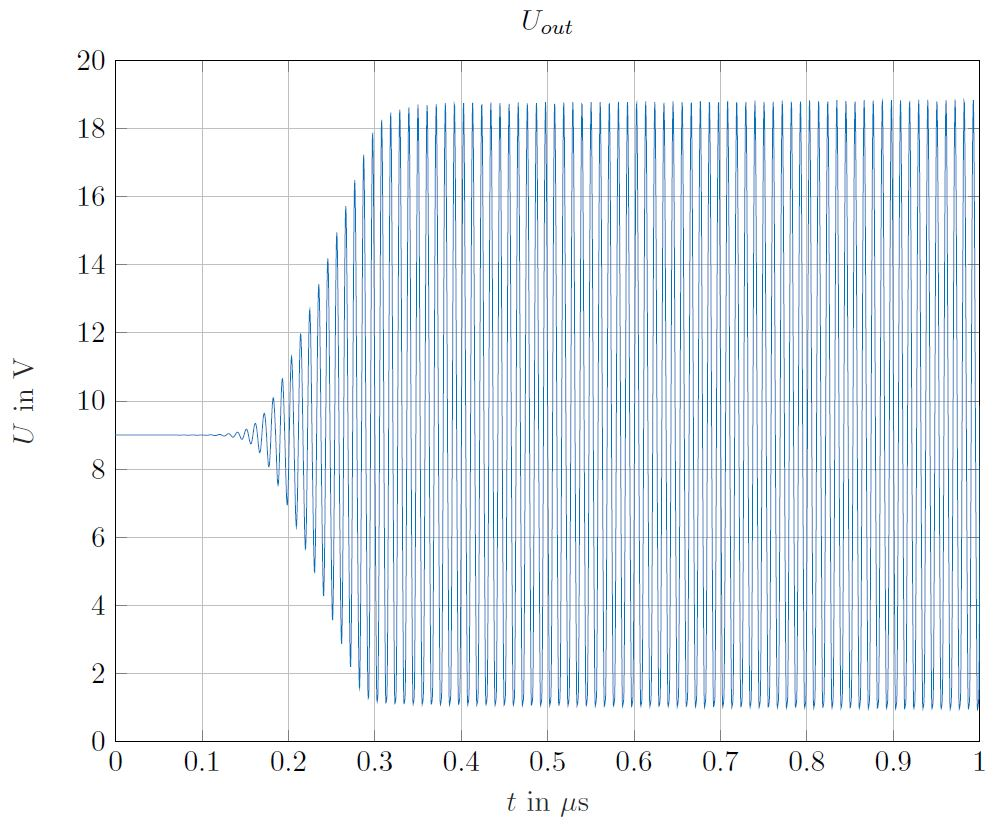
\includegraphics[width = 0.8\textwidth]{\figpath/U_out_LC_oszi_inter.jpg}
	\caption{Ausgangsspannung des Oszillators}
	\label{fig_Kap2_06:Uout}
\end{figure}

Als nächstes wird der Einschwingvorgang weggeschnitten, d.h. die Ausgangsspannung im Zeitbereich von $\SI{1}{\micro\second}$ bis $\SI{2}{\micro\second}$ betrachtet und davon die FFT gebildet. In Abb. \ref{fig_Kap2_07:FFT} wird einmal die FFT des Oszillatorsignals bei $\SI{2}{\micro\second}$ (short) und einmal bei $\SI{10}{\micro\second}$ (long) Simulationszeit dargestellt. Es stellt sich heraus, dass die Simulationsdauer in diesem Fall erheblichen Einfluss auf das Ergebnis der FFT hat. Die Resonanzfrequenz liegt bei längerer Simulationsdauer im Vergleich etwas höher und ist um ein schmaleres Frequenzband ausgeprägt, was letztendlich in einem höheren Gütefaktor resultiert. Der Grund für diesen Effekt liegt in den Fehlern der numerischen Berechnungen, die der Simulation zu Grunde liegen.

\begin{figure}[H]
    \centering
    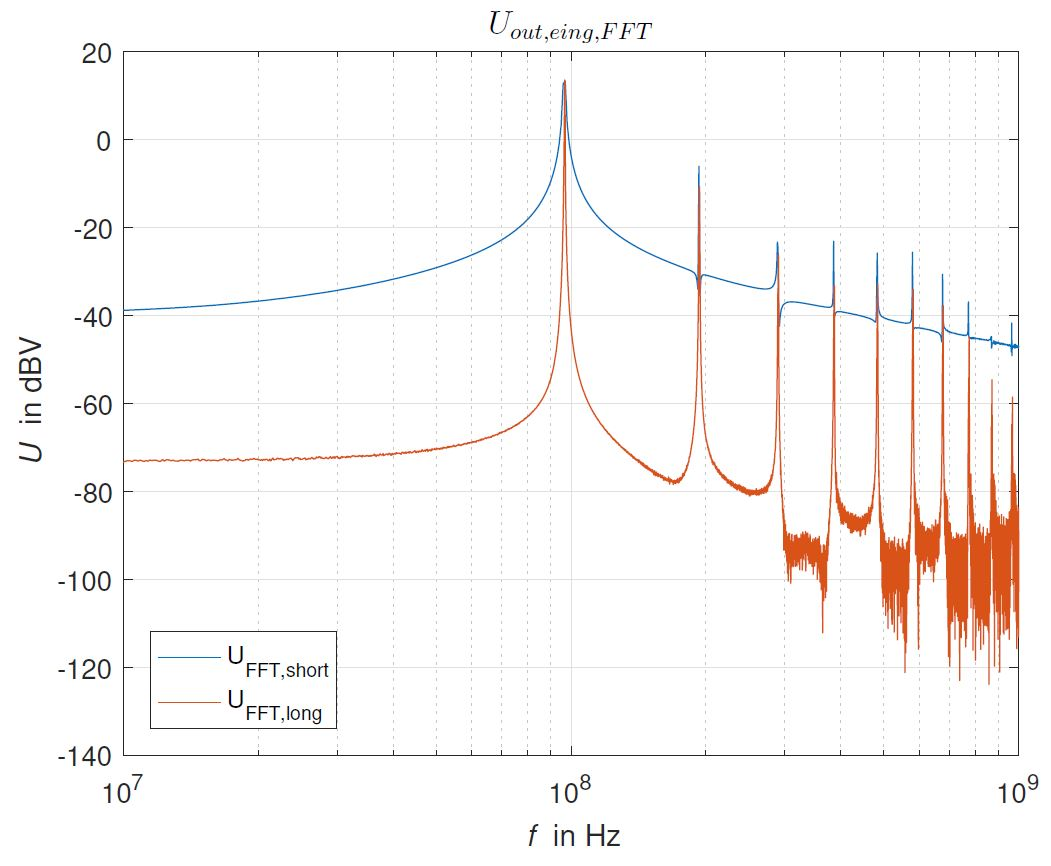
\includegraphics[width = 0.8\textwidth]{\figpath/U_FFT.jpg}
    \caption{FFT der Ausgangsspannung ohne Einschwingvorgang}
    \label{fig_Kap2_07:FFT}
\end{figure}

Mithilfe der Vergrößerung um den Resonanzbereich kann nun die Bandbreite und der Gütefaktor des Oszillators bestimmt werden. Der Zusammenhang des Gütefaktors $Q$, der Resonanzfrequenz $f_0$ und der 3dB-Bandbreite $B$ lautet folgendermaßen:

\begin{equation}
    Q = \frac{f_0}{B}
\end{equation}

Für die kurze Simulationsdauer ergeben sich folgende Werte:

\begin{equation*}
    f_0 = \SI{95}{\mega\hertz}
\end{equation*}

\begin{equation*}
    B = f_2 - f_1 = \SI{95.36}{\mega\hertz} - \SI{94.66}{\mega\hertz} = \SI{0.7}{\mega\hertz}
\end{equation*}

\begin{equation*}
    Q = \frac{f_0}{B} = \frac{95}{0.7} = 135.7
\end{equation*}

Für die lange Simulationsdauer ergibt sich eine etwas höhere Resonanzfrequenz und eine höhere Güte.

\begin{equation*}
    f_0 = \SI{95.8}{\mega\hertz}
\end{equation*}

\begin{equation*}
    B = f_2 - f_1 =  = \SI{95.95}{\mega\hertz} - \SI{95.7}{\mega\hertz} = \SI{0.25}{\mega\hertz}
\end{equation*}

\begin{equation}
    Q = \frac{f_0}{B} = \frac{95.8}{0.25} = 383.2
\end{equation}

Als nächstes wird die Abhängigkeit der Resonanzfrequenz vom Arbeitspunkt des Transistors untersucht. Hierzu wurde der Widerstand $R_1$ variiert und über Simulation die Resonanzfrequen ermittelt. Die Werte wurden in Tab. eingetragen sowie als Diagramm in Abb. \ref{fig_Kap2_09:AP} dargestellt.

\begin{table}[H]
\centering
\begin{tabular}{|c|c|c|} \hline
$R_1$ in k$\Omega$ & $U_L$ in V & $f_0$ im MHz \\ \hline
27 & 0.596 & 96.5 \\ \hline
15 & 0.628 & 96 \\ \hline
10 & 0.642 & 95.5 \\ \hline
2.7 & 0.674 & 92 \\ \hline
1 & 0.687 & 87.10 \\ \hline
\end{tabular}
\caption{Variation des AP und Resonanzfrequenz}
\label{tab_Kap2_02:AP} 
\end{table}

\begin{figure}[H]
	\centering \small
	% This file was created by matlab2tikz.
%
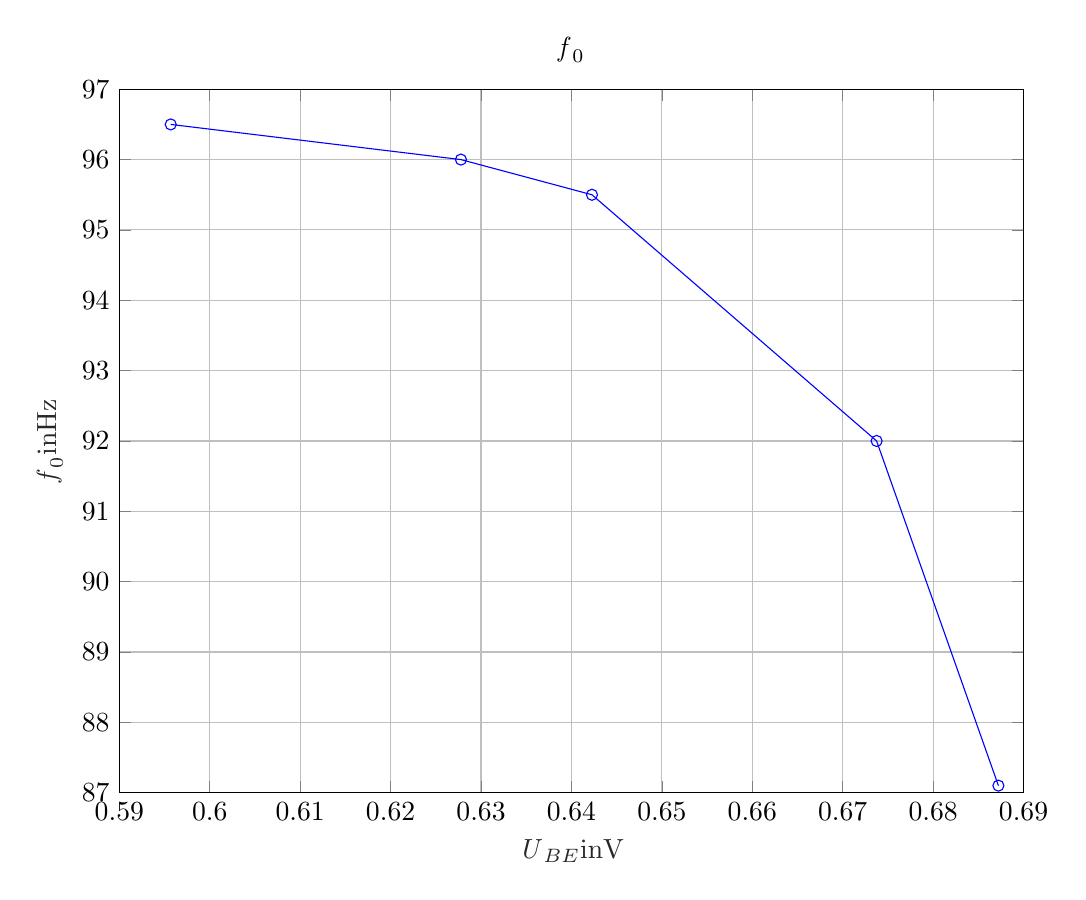
\begin{tikzpicture}

\begin{axis}[%
width=4.521in,
height=3.517in,
at={(0.758in,0.519in)},
scale only axis,
xmin=0.59,
xmax=0.69,
xlabel style={font=\color{white!15!black}},
xlabel={$\text{\it{} U}_{\text{BE}}\text{ \rm{} in V}$},
ymin=87,
ymax=97,
ylabel style={font=\color{white!15!black}},
ylabel={$\text{\it{} f}_\text{0}\text{ \rm{} in Hz}$},
axis background/.style={fill=white},
title style={font=\bfseries},
title={$\text{\it{} f}_{\text{0}}$},
xmajorgrids,
ymajorgrids
]
\addplot [color=blue, mark=o, mark options={solid, blue}, forget plot]
  table[row sep=crcr]{%
0.68722	87.1\\
0.67375	92\\
0.64227	95.5\\
0.627778	96\\
0.595685	96.5\\
};
\end{axis}
\end{tikzpicture}%
	\caption{$f_0$ in Abhängigkeit des AP}
	\label{fig_Kap2_09:AP}
\end{figure}

Die Abhängigkeit der parasitären Kapazitäten vom Arbeitspunkt des Transistors führen dazu, dass sich die Resonanzfrequenz des Oszillators gemeinsam mit dem Arbeitspunkt verändert. In Kombination mit dem Mikrofonverstärker könnte dieser Effekt dazu genutzt werden, einen Mono-FM-Sender zu realisieren.



